% !TeX spellcheck = en_US
\chapter{Meta-Learning}

\section{Scaffolding}
\textit{Scaffolding} is a term that commonly used in the construction field, but also has a relation to infant's learning process. Scaffolding is a temporary structure that supports the construction, maintenance of a large building \href{https://en.wikipedia.org/wiki/Scaffolding}{(wiki)}. In the context of learning, it implies the structured assistance, or guidance, for better accomplishment of new skills and tasks. As the learner's \textit{autonomy} (learning abilities) increases, the support decrease accordingly . \cite{parentlab2019ccaffolding, zaadnoordijk2020next}

\begin{figure}[hbt!]
	\centering
	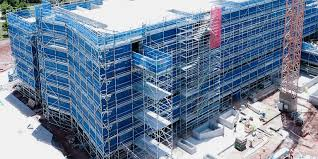
\includegraphics[width=.5\textwidth]{scaffolding.jpeg}
	\caption{Scaffolding in construction.}
\end{figure}

Extending the idea behind scaffolding to \ac{ML} and \ac{RL}: \cite{zaadnoordijk2020next}
\begin{itemize}
	\item Visual imitation learning \cite{finn2017one, sharma2019third}
	\item Learning from demonstration \todo{}
	\item Collective learning: learn from / guided by other agents
	\item Active learning
\end{itemize}

\todo{Read \cite{soltoggio2018born, arandjelovic2017look, barros2019expectation}}

\todo{Read \href{https://www.deepmind.com/publications/a-generalist-agent}{A Generalist Agent}}

\todo{Read \href{https://research.facebook.com/publications/control-strategies-for-physically-simulated-characters-performing-two-player-competitive-sports/}{meta}}

\section{Learning Resource}
\begin{itemize}
	\item \href{https://youtu.be/ByeRnmHJ-uk}{Learning to learn: An Introduction to Meta Learning || \ac{ICML} 2019}
\end{itemize}

\section{Definitions}
Conventional supervised learning relies on large and diverse dataset for broad generalization. There are, however, problems with limited labeled data. These scenarios would need a general purpose \ac{AI} system to adapt and learn on the job.

\begin{center}
	\begin{tabular}{p{8cm}|p{8cm}}
		Mechanistic view & Probabilistic view\\
		\hline\hline
		- Deep neural network model that can read in an entire dataset and make predictions for new datapoints  & - Extract prior information from a set of (meta-training) tasks that allows efficient learning of new tasks\\
		- Training this network uses a meta-dataset, which itself consists of many datasets, each for a different task & - Learning a new task uses this prior and (small) training set to infer most likely posterior parameters\\
		- Easier to implement meta-learning & - Easier to understand meta-learning
	\end{tabular}
\end{center}

\begin{itemize}
	\item If you’ve learned 100 tasks already, can you figure out how to learn more efficiently?
	\item Meta-learning = learning to learn
	\item In practice, very closely related to multi-task
	\item A meta-learned learner can:
	\begin{itemize}
		\item Explore more intelligently
		\item Avoid trying actions that are known to be useless
		\item Acquire the right features more quickly
	\end{itemize}
\end{itemize}

\section{Supervised Meta-learning}
The problem setup (\figref{fig:supervised-meta-learning}):
\begin{itemize}
	\item Meta-training: acquire your learned learning algorithm
	\item Meta-testing: use/adapt your learned learning algorithm
	\item Meta-training and meta-testing have separated training data and test data
\end{itemize}

\begin{figure}[hbt!]
	\centering
	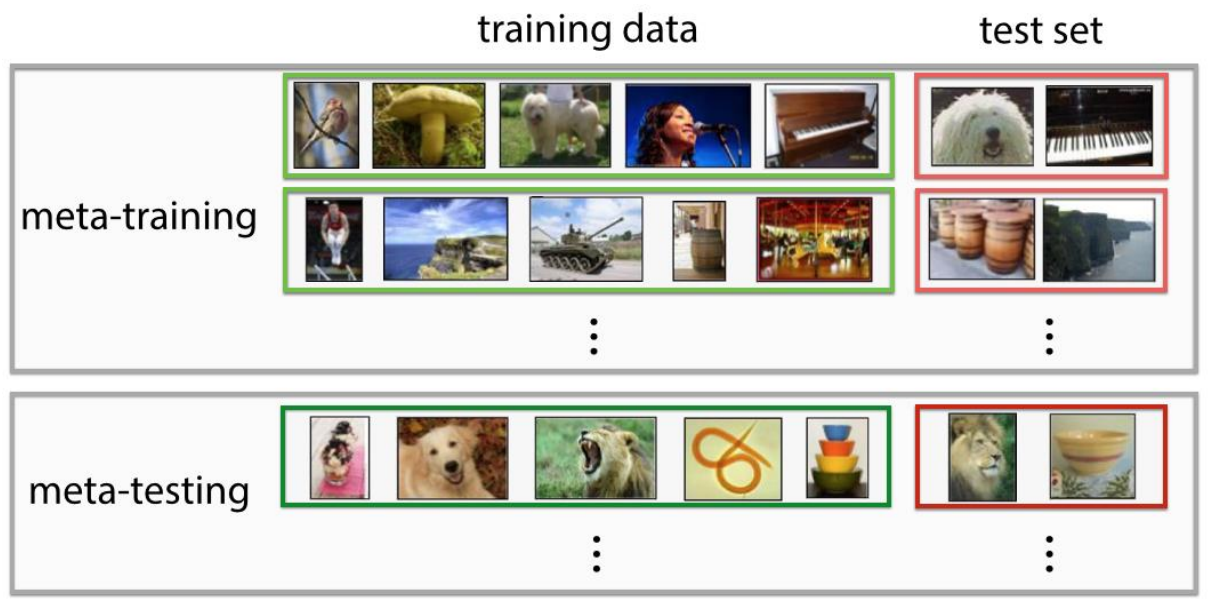
\includegraphics[width=.7\textwidth]{supervised-meta-learning.png}
	\caption{Supervised meta-learning pipeline (Ravi \& Larochelle '17)}
	\label{fig:supervised-meta-learning}
\end{figure}

\begin{multicols}{2}
	Supervised learning:
	\begin{align*}
		&f(x) \rightarrow y\\
		&\underset{\phi}{\arg\max} \log p(\phi | \mathcal{D})
	\end{align*}	
	Supervised meta-learning:
	\begin{align*}
		&f(\mathcal{D}^{tr}, x) \rightarrow y\\
		&\underset{\phi}{\arg\max} \log p(\phi | \mathcal{D}, \mathcal{D}_{meta-train})
	\end{align*}
\end{multicols}
\begin{align*}
	&x &&-\text{input}\\
	&y &&-\text{output}\\
	&\mathcal{D} = \{(x_1, y_1), \dots, (x_k, y_k)\} &&-\text{dataset}\\
	&\mathcal{D}_{meta-train} = \{(\mathcal{D}_1^{tr}, \mathcal{D}_1^{ts}), \dots, (\mathcal{D}_n^{tr}, \mathcal{D}_n^{ts})\} &&-\text{meta dataset}\\
	&\mathcal{D}_i = \{(x_1^i, y_1^i), \dots, (x_k^i, y_k^i)\}
\end{align*}

\begin{figure}[hbt!]
	\centering
	\begin{tikzpicture}[
		recnode1/.style={rectangle, draw=black!72, very thick, minimum width=1cm, minimum height=5mm},
		recnode2/.style={rectangle, minimum size=5mm}]
		\node[recnode1](x1){};
		\node[recnode1](x2)[right=of x1]{};
		\node[recnode1](x3)[right=of x2]{};
		\node[recnode1](x4)[right=of x3]{};
		\node[recnode2](y1)[below=0.5cm of x1]{$(x_1, y_1)$};
		\node[recnode2](y2)[below=0.5cm of x2]{$(x_2, y_2)$};
		\node[recnode2](y3)[below=0.5cm of x3]{$(x_3, y_3)$};
		\node[recnode2](y41)[below=0.5cm of x4]{$x_{test}$};
		\node[recnode2](y42)[above=0.5cm of x4]{$y_{test}$};
		\draw[-latex] (x1.east) -- (x2.west);
		\draw[-latex] (x2.east) -- (x3.west);
		\draw[-latex] (x3.east) -- (x4.west);
		\draw[-latex] (y1.north) -- (x1.south);
		\draw[-latex] (y2.north) -- (x2.south);
		\draw[-latex] (y3.north) -- (x3.south);
		\draw[-latex] (y41.north) -- (x4.south);
		\draw[-latex] (x4.north) -- (y42.south);
	\end{tikzpicture}
	\caption{Using \ac{RNN} to input a training set $\mathcal{D}^{tr}$, instead of just $x$.}
\end{figure}

The knowledge from the meta training dataset $\mathcal{D}_{meta-train}$ is extracted into parameter $\theta$:
\begin{align}
	&\theta^* = \underset{\theta}{\arg\max} \log p(\theta | \mathcal{D}_{meta-train}) && -\text{meta-learning} \\
	&\log p(\phi | \mathcal{D}, \mathcal{D}_{meta-train}) \approx \log p(\phi | \mathcal{D}, \theta^*)\\
	&\phi^* = \underset{\phi}{\arg\max} \log p(\phi | \mathcal{D}, \theta^*) && -\text{adaptation}
\end{align}

\begin{figure}[hbt!]
	\centering
	\begin{subfigure}[b]{0.45\textwidth}
		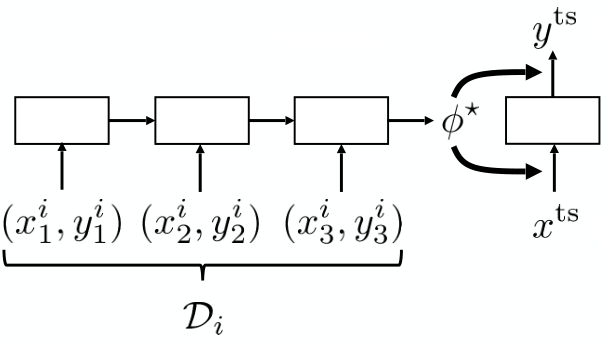
\includegraphics[width=\textwidth]{meta-training.png}
		\caption{Meta-training: $(x^{ts}, y^{ts}) \sim \mathcal{D}_i^{ts}$}
	\end{subfigure}
	\hfil
	\begin{subfigure}[b]{0.45\textwidth}
		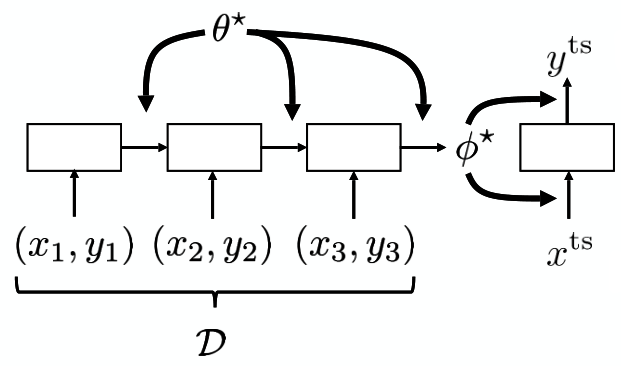
\includegraphics[width=\textwidth]{meta-testing.png}
		\caption{Meta-testing}
	\end{subfigure}
	\caption{Matching test and train conditions.}
\end{figure}

\begin{align}
	\phi^* = f_{\theta^*} (\mathcal{D}^{tr})
\end{align}

\todo{still confusing}

\begin{itemize}
	\item In meta-training, each task has a training set $\mathcal{D}^{tr}_i$ and a test set $\mathcal{D}^{ts}_i$.
	\item $\phi_i$ is the \ac{param} learned from the task's training set $\mathcal{D}^{tr}_i$ (\figref{fig:rnn-meta-learning}).\\
	$\phi_i = [h_i, \theta_p]$ with $h_i$ - \ac{RNN} hidden state, $\theta_p$ - meta-learned weights.
	\item In meta-testing, we optimize $\theta$, which is the $\arg\min$ of the average over all the tasks (in meta-training), of the loss of that task on its test set $\mathcal{D}^{ts}_i$.
\end{itemize}
\note The test set in meta-testing is not available (of course) for learning $\theta$, but the test set for meta-training is (\figref{fig:supervised-meta-learning}).

\begin{figure}[hbt!]
	\centering
	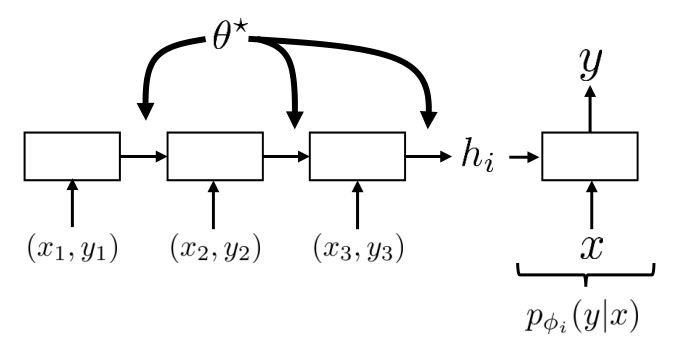
\includegraphics[width=.45\textwidth]{rnn-meta-learning.png}
	\caption{$\phi_i = [h_i, \theta_p]$ (\href{http://rail.eecs.berkeley.edu/deeprlcourse/static/slides/lec-22.pdf}{src})}
	\label{fig:rnn-meta-learning}
\end{figure}

\section{Meta Reinforcement Learning}
\begin{multicols}{2}
	Reinforcement learning:
	\begin{align*}
		\theta^* &= \underset{\theta}{\arg\min} \mathbb{E}_{\pi_\theta(\tau)} [R(\tau)]\\
		&= f_{RL}(\mathcal{M})\\
		&\mathcal{M} = \{\mathcal{S, A, P}, r\}:\;\text{the \ac{MDP}}
	\end{align*}
	Meta-reinforcement learning:
	\begin{align*}
		\theta^* &= \underset{\theta}{\arg\min} \sum_{i=1}^n \mathbb{E}_{\pi_{\phi_i}(\tau)} [R(\tau)]\\
		&\text{where}\; \phi_i = f_\theta(\mathcal{M}_i)\\
		&\mathcal{M}_i:\;\text{the \ac{MDP} for task $i$}
	\end{align*}
\end{multicols}

\begin{align}
	\mathcal{M}_i \sim p(\mathcal{M})\\
	\mathcal{M}_{test} \sim p(\mathcal{M})
\end{align}

\begin{itemize}
	\item In multi-task \ac{RL}, the context is typically given.
	\item In meta-\ac{RL}, the \textit{context} is inferred from experience from $\mathcal{M}_i$: $\pi_\theta(a_t | s_t, \phi_i)$
\end{itemize}

\section{Gradient-based Meta Learning}

\note The word \textit{agnostic} implies that some characteristics are irrelevant and that something is widely applicable. \Eg, a pick and place strategy is object-agnostic, if it doesn't matter what characteristics the object has, classes, geometries, materials, \etc. In other words, that strategy is compatible to a variety of objects.

\hlb{Idea:} pretraining as a type of meta-learning.\\
In \ac{MAML}, $f_\theta(\mathcal{M}_i)$ is itself an \ac{RL} \ac{algor} \cite{finn2017model}

\begin{align}
	\theta^* &= \arg\max \sum_{i=1}^n \mathbb{E}_{\pi_{\theta_i}} [r(\tau)]\\
	&\text{where}\; \phi_i = f_\theta(\mathcal{M}_i)\\
	f_\theta(\mathcal{M}_i) &= \theta + \alpha \nabla_\theta J_i(\theta)
\end{align}

\begin{align}
	&\cancel{\theta \leftarrow \theta + \alpha \nabla_\theta J(\theta)}\\
	&\theta \leftarrow \theta + \beta \sum_i \nabla_\theta J_i[\theta + \alpha \nabla_\theta J(\theta)]
\end{align}

\section{Meta-RL as a POMDP}
\subsection{PEARL}
\subsection{MELD}

\section{Model-Based Meta-RL}

\section{Meta-RL and Emergent Phenomena}
Humans and animals learn behaviors in a variety of ways. Perhaps each is a separate algorithm in the brain. But maybe these are all emergent phenomena resulting from meta-\ac{RL}:
\begin{itemize}
	\item Highly efficient but (apparently) model-free RL
	\item Episodic recall
	\item Model-based RL
	\item Causal inference
	\item etc.
\end{itemize}

References:
\begin{itemize}
	\item \citeaustitle{ritter2018been}
	\item \citeaustitle{wang2018prefrontal}
	\item \citeaustitle{dasgupta2019causal}
\end{itemize}

\section{References}
\hlb{Gradient-based Meta-RL}

\ac{MAML} meta-policy gradient estimators:
\begin{itemize}
	\item \citeaustitle{finn2017model}
	\item \citeaustitle{foerster2018dice}
	\item \citeaustitle{rothfuss2018promp}
\end{itemize}

Improving exploration:
\begin{itemize}
	\item \citeaustitle{gupta2018meta}
	\item \citeaustitle{stadie2018some}
\end{itemize}
	
Hybrid algorithms (not necessarily gradient-based):
\begin{itemize}
	\item \citeaustitle{houthooft2018evolved}
	\item \citeaustitle{fernando2018meta}
\end{itemize}

\hlb{Meta-RL, Inference, and POMDPs}
\begin{itemize}
	\item \citeaustitle{rakelly2019efficient}
	\item \citeaustitle{zintgraf2019variational}
	\item \citeaustitle{humplik2019meta}
	\item \citeaustitle{liu2020explore}
\end{itemize}
